% -*- root: ../thesis.tex -*-
%!TEX root = ../thesis.tex

% ******************************* Thesis Chapter 1 ****************************

% the code below specifies where the figures are stored
\ifpdf
    \graphicspath{{chapters/1_introduction/figures/}}
\else
    \graphicspath{{1_introduction/figures/EPS/}{1_introduction/figures/}}
\fi
% ----------------------------------------------------------------------
%: ----------------------- introduction content ----------------------- 
% ----------------------------------------------------------------------

\ac{ML} is a wide field of research with plenty of successful applications, in particular with domains such as computer vision, natural language processing, or reinforcement learning \cite{jordan2015machine}.
A particular branch of interest is \textbf{probabilistic} machine learning.
Probabilistic \ac{ML} defines quantities of interest as random variables and considers processes as stochastic.
We can build more flexible and robust models using paradigms and tools from statistics.
It produces complete and rich results and helps connect with classical sciences such as physics or climatology, where statistical analysis is standard practice.\mycom{rework with whole part}

\section{Bayesian Machine Learning}

Some real-world problems have critical requirements.
For example, predictive probability guarantees and meaningful uncertainties are essential for decision-making algorithms.
The Bayesian framework addresses both these aspects by working with \textbf{random variables} defined by \textbf{probability distributions} instead of point estimates.
For a given probabilistic model, by setting a \textbf{prior distribution} over the parameters of interest, the \textbf{posterior distribution} represents the updated belief we have about our model after observing data.
Probabilistic models allow modeling uncertainty in a principled way and prevent overfitting in the low-data regime.
A typical example is in medicine, where data is scarce, but the predictive outcome can have dramatic effects (diagnosis, prognosis).
Providing uncertainties helps the practitioner make a decision given the model predictions.

Generally, Bayesian models have a higher computational cost: a probability distribution contains more information than a point estimate and requires more parameters.
Calculus with random variables is a complex science, and finding analytical solutions happens almost exclusively for trivial models.
Approximation methods allow working with more complex models at the cost of lower accuracy. 
\textbf{\ac{ABI}} focuses on these algorithms finding a similar solution to the true posterior.

The research in \ac{ABI} goes in many directions, but some main ones are: How to compute a highly accurate posterior approximation as efficiently as possible? How can it scale to large amounts of data and parameters? What are the guarantees of such algorithms?
This thesis aims to partially answer these questions for some given setups, mainly through the lens of model representation.

\section{The underestimated power of representations choices}

% \begin{itemize}
%     \item Different representation lead to very different results, efficiency etc.
%     \item Mention existing approaches
% \end{itemize}
The leading thread of this thesis is \textbf{model representation}, alternatively called \textbf{model parameterization}, and its use for solving problems more efficiently and faster without compromising prediction quality.

When defining probabilistic models, one needs to define relations between variables (observed and latent) and choose appropriate distributions to represent those.
Some modeling choices are equivalent conceptually but have drastic differences in inference.
A neat example, presented in \citet{gorinovaAutomaticReparameterisationProbabilistic2020}, is the so-called Neal's funnel.
There are two equivalent representations, called centered and non-centered, shown respectively in Figure~\ref{fig:neals_centered} and~\ref{fig:neals_noncentered}, where one leads to an inference nightmare while the other is a nice and easy isotropic Gaussian distribution.

\begin{minipage}{0.5\textwidth}
    \centering
    \begin{align}
        \begin{aligned}
            z \sim&\; \mathcal{N}(0, 3)\\
            x \sim&\; \mathcal{N}(0, \exp(z/2))
        \end{aligned}
    \end{align}
    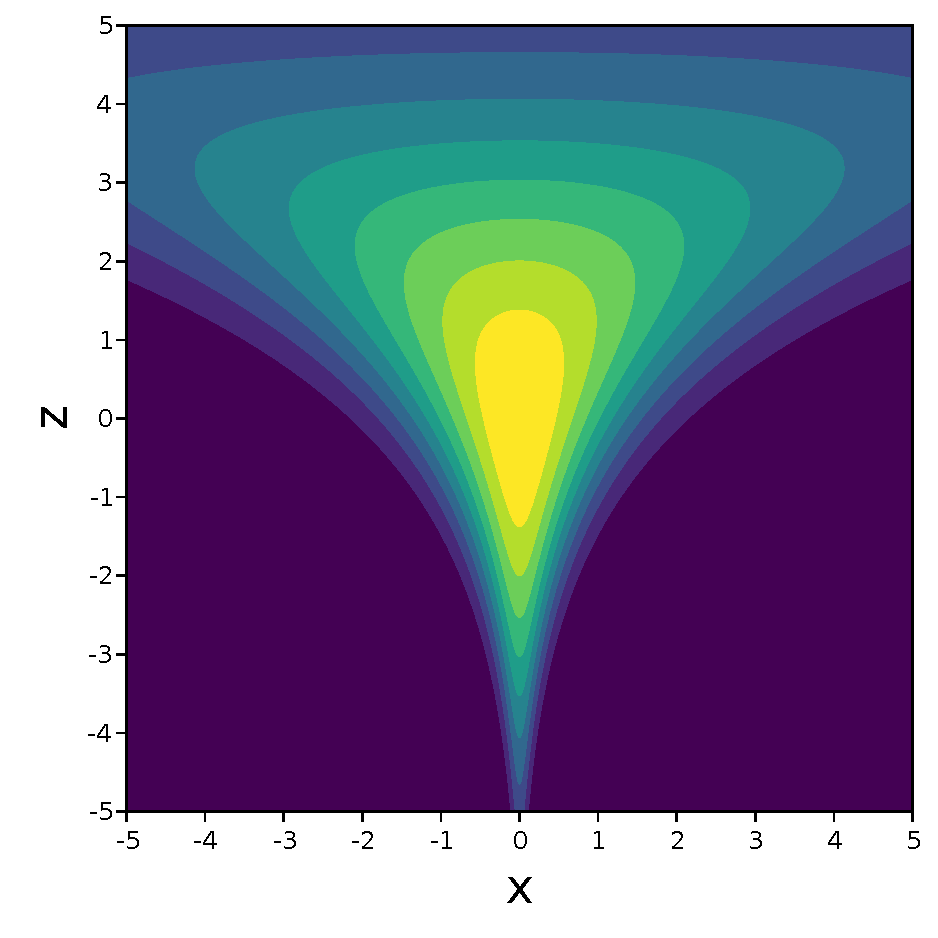
\includegraphics[width=\textwidth]{./chapters/1_introduction/figures/neals_funnel_centered.pdf}
    \captionof{figure}{Neal's funnel - Centered representation}
    \label{fig:neals_centered}
\end{minipage}
\begin{minipage}{0.5\textwidth}
    \centering
    \begin{align}
        \begin{aligned}
            \tilde{z} \sim&\; \mathcal{N}(0, 1),\quad z = 3\tilde{z}\\
            \tilde{x} \sim&\; \mathcal{N}(0, 1),\quad x = \exp(z/2)\tilde{x}
        \end{aligned}
    \end{align}
    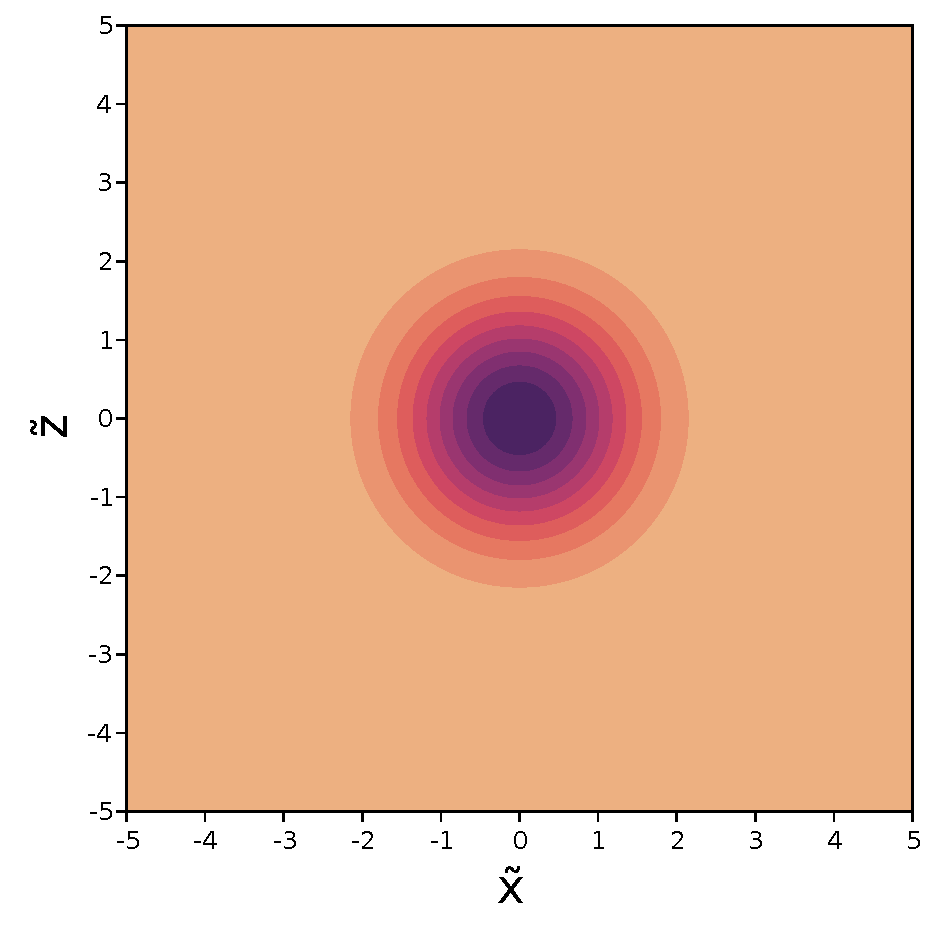
\includegraphics[width=\textwidth]{./chapters/1_introduction/figures/neals_funnel_non_centered.pdf}
    \captionof{figure}{Neal's funnel - Non-centered representation}
    \label{fig:neals_noncentered}
\end{minipage}
\vspace{0.5cm}

While both parameterizations are the same, the distribution geometry of $p(x,z)$ is less favorable to inference.
$x$ and $z$ are highly correlated for small $z$s, and the distribution function is highly non-smooth.
These constraints matter when running a sampling chain or fitting a variational distribution.
% An analogy in physics would be how easier it is to work with spherical coordinates instead of Euclidean ones for electrodynamics. 

Using different model representations has an often underestimated effect and is mainly considered "tricks".
For example, when working with \acf{GPs}, it is preferable to use the so-called "whitened" representation, which corresponds to our non-centered representation of Neal's funnel.
The different segments of this thesis show that finding better representations can confidently make inference easier, faster, and significantly more stable. 
The first part will use basic inference methods by representing likelihoods as (hierarchical) mixtures.
Defined later in Section \ref{sec:scale-mixtures}, rewriting distributions as scale-mixtures has a lot of advantages and interesting properties.
The scale-mixtures representation involves augmenting the model with new latent variables, making inference easier while keeping the original model recoverable.
This augmentation procedure brings the counter-intuitive view that adding more variables \textbf{simplifies} the problem.
The last work of the thesis focuses on the representation of the variational Gaussian approximation.
We avoid computational bottlenecks and add flexibility using a non-conventional approach based on particles.

\section{Gaussian Processes}

The techniques mentioned above apply to many probabilistic models; however, we focus strongly on Gaussian-based models, and more particularly \acf{GPs}.
A \ac{GP} is a strong non-parametric tool to approximate functions using probabilistic methods.
They were originally applied to Gaussian regression problems, like the original \textbf{kriging problem} \cite{cressie1990origins}. However, they can also be used as latent functions for more complex problems like classification, ordinal regression, and more.
Compared to other general function approximators like neural networks, they have the advantage of providing uncertainty on the prediction they make.
Their non-parametric nature naturally avoids over-parametrization: while modern neural networks have billions of parameters to optimize, \ac{GPs} only depend on a mean function and a kernel function.
Most importantly, as their name suggests, they are based on Gaussian distributions, making them the best candidates for the presented work on augmentation.
A full technical introduction to basic \ac{GPs} and its extensions is given in Section~\ref{sec:gps}.

\section{Open-source projects}

All the works presented in this thesis, as well as additional tools, are backed-up by user-friendly packages in Julia \cite{Julia-2017}.
Throughout my time as a Ph.D. student, I have developed numerous Julia packages and was involved in the \href{https://github.com/JuliaGaussianProcesses}{JuliaGaussianProcesses organisation} to develop a flexible, efficient and easy-to-use framework to work with \ac{GPs} from the very low-end to high-end interfaces through a series of packages: \href{https://github.com/JuliaGaussianProcesses/KernelFunctions.jl}{KernelFunctions.jl}~\cite{theo_galy_fajou_2022_6246597}, \href{https://github.com/JuliaGaussianProcesses/AbstractGPs.jl}{AbstractGPs.jl}~\cite{david_widmann_2022_5939997}, \href{https://github.com/JuliaGaussianProcesses/ApproximateGPs.jl}{ApproximateGPs.jl} and \href{https://github.com/JuliaGaussianProcesses/GPLikelihoods.jl}{GPLikelihoods.jl}.
The particular strength of our work is the one-to-one mapping between theory and code.
For example to define the posterior for some given data, the code looks like:
\begin{minted}[breaklines,escapeinside=||,mathescape=true, numbersep=3pt, gobble=2, frame=lines, fontsize=\small, framesep=2mm]{julia}
    f = GP(mean_prior, kernel) # define an infinite-dimensional prior
    fx = f(X, noise) # create a realization on the data X
    fpost = posterior(fx, y) # Create the posterior given the observations y
\end{minted}
Here, each computational object represents exactly its mathematical equivalent.

The work of this thesis is represented as well with the package \href{https://github.com/JuliaGaussianProcesses/AugmentedGPLikelihoods.jl}{AugmentedGPLikelihoods.jl}, which provide all the necessary tools to work with augmentations.
Julia's advantage is its strong interoperability capacity.
This allows to use the augmentation work on specific implementation of \ac{GPs} such as temporal \ac{GPs} with a concrete example given in \href{https://github.com/JuliaGaussianProcesses/TemporalGPs.jl}{TemporalGPs.jl} (see examples/augmented\_inference.jl).

Independently, I also developed \href{https://github.com/theogf/AugmentedGaussianProcesses.jl}{AugmentedGaussianProcesses.jl}~\cite{theo_galy_fajou_2021_5728215} as a stand-alone \ac{GP} package providing the augmentations techniques presented in the thesis, additional likelihoods and standard inference approaches.

\section{Thesis Outline}

This thesis is constructed as follows:
\begin{itemize}
    \item Chapter~\ref{ch:background} introduces in details all the common concepts of Bayesian inference and \ac{GPs}.
    There are introductions to these concepts in each published article, but this chapter dives more into the background theory.
    Bayesian inference, especially, is properly introduced, focusing on variational inference and sampling.
    \item Chapter~\ref{ch:classification} contains the paper \textit{Efficient Gaussian Process Classification Using P\`olya-Gamma Data Augmentation}, which was the first augmentation we explored.
    \item Chapter~\ref{ch:multiclass} introduced the paper \textit{Multi-Class Gaussian Process Classification Made Conjugate: Efficient Inference via Data Augmentation}.
    This paper brings new augmentation concepts to a more complex problem: multi-class classification.
    \item Chapter~\ref{ch:general} introduces the paper \textit{Automated Augmented Conjugate Inference for Non-conjugate Gaussian Process Models}.
    This work is the first generalization of augmentation identification and allows getting a better understanding of these concepts.
    \item Chapter~\ref{ch:gpf} introduces the paper \textit{Flexible and Efficient Inference with Particles for the Variational Gaussian Approximation } a completely different way of performing variational inference with a Gaussian distribution by using a continuous flow and particles.
    \item Chapter~\ref{ch:discussion} discusses the different papers presented as well as some concrete outlooks on how to explore new models and new generalizations.
    \item Chapter~\ref{ch:conclusion} finishes this thesis with a general conclusion.
    \item The Appendix~\ref{appendix:worshoppapers} also contains an additional workshop paper which do not fit the narrative of this thesis 

    For all papers, the contribution will be detailed using a simplified view of the \href{https://mdpi-res.com/data/contributor-role-instruction.pdf}{Contributor Roles Taxonomy} (CReditT).

\end{itemize}

